\documentclass[conference]{IEEEtran}
\IEEEoverridecommandlockouts
\usepackage{cite}
\usepackage{amsmath,amssymb}
\usepackage{graphicx}
\usepackage{booktabs}
\usepackage{multirow}
\usepackage{xcolor}
\usepackage{tikz}
\usetikzlibrary{arrows.meta,positioning,fit}
\usepackage[hidelinks]{hyperref}
\usepackage{url}
\def\BibTeX{{\rm B\kern-.05em{\sc i\kern-.025em b}\kern-.08em
    T\kern-.1667em\lower.7ex\hbox{E}\kern-.125emX}}

\begin{document}

\title{CloudChain: Attack-Path Analysis for AWS with\\Read-Only Validation Against the Live Account}

\author{
\IEEEauthorblockN{Parth Joshi}
\IEEEauthorblockA{\textit{Symbiosis Skills and Professional University}\\
Pune, India}
\and
\IEEEauthorblockN{Hrishikesh Kanapuram}
\IEEEauthorblockA{\textit{Symbiosis Skills and Professional University}\\
Pune, India}
\and
\IEEEauthorblockN{Aaryaman Bhatnagar}
\IEEEauthorblockA{\textit{Symbiosis Skills and Professional University}\\
Pune, India}
\and
\IEEEauthorblockN{Saahithi Mukala}
\IEEEauthorblockA{\textit{Symbiosis Skills and Professional University}\\
Pune, India}
\and
\IEEEauthorblockN{Dr. Sunil Kale}
\IEEEauthorblockA{\textit{Symbiosis Skills and Professional University}\\
Pune, India}
}

\maketitle

\begin{abstract}
Cloud security posture management (CSPM) tools usually report AWS misconfigurations as a flat list, one check at a time. Breaches tend to come from chains of weaknesses instead, and the tools that do model chains derive them from configuration and present them as fact. We describe CloudChain, an open-source CSPM tool that builds a graph of AWS resources and identities, searches it for routes to administrator access, and then re-checks every hop of every route against the live account using read-only API calls. For permission hops it asks AWS's own policy simulator, which applies explicit denies, permissions boundaries and service control policies (SCPs) that static analysis does not model. Each hop comes back CONFIRMED, REFUTED or UNVERIFIABLE, together with the API calls behind the verdict. We evaluated CloudChain on a real AWS account governed by an organisation SCP, using nine IAM test identities with known ground truth. CloudChain and Prowler both flagged all six escalation-capable identities and none of the three negative controls. Validation then showed that four of the seven routes CloudChain derived (57\%) could not be walked because the SCP denied an action they depended on, a distinction Prowler's output does not make. After we removed the escalation permission from two identities, re-validating the stored scan marked exactly those two routes REFUTED. On synthetic organisations the analysis took 2.6\,s for 10{,}000 identities, and a hop limit kept path search bounded on dense graphs where unbounded enumeration exceeded 60\,s at 10 identities.
\end{abstract}

\begin{IEEEkeywords}
cloud security, AWS IAM, attack graphs, privilege escalation, security posture management, policy validation
\end{IEEEkeywords}

\section{Introduction}

Free CSPM tools such as Prowler~\cite{prowler} and ScoutSuite~\cite{scoutsuite} run hundreds of independent checks against an AWS account and report each failure with a fixed severity. A public bucket, a user without MFA and a policy that grants \texttt{iam:PassRole} appear as separate rows. An attacker sees them differently: the bucket exposes a key, the key belongs to the user, and the user can pass an administrator role into a new Lambda function. The risk is the chain, and a flat list hides it.

Graph-based tools address this. PMapper~\cite{pmapper} and awspx~\cite{awspx} model IAM principals and the edges between them, and commercial products present attack paths on a dashboard. These paths are still outputs of a model built from configuration. A path can look complete and still be blocked by an SCP, a permissions boundary or an explicit deny that the analyser never read. Security teams that have seen enough blocked paths learn to distrust the whole category of finding.

CloudChain treats a reported path as a claim to be tested. This paper makes four contributions:
\begin{enumerate}
\item A resource graph for AWS that separates same-account \texttt{iam:PassRole} escalation from cross-account \texttt{sts:AssumeRole} movement, so that no reported chain crosses an account boundary through a mechanism AWS does not allow (Section~\ref{sec:design}).
\item A read-only validation engine that re-checks each hop of each path against the live account and consults \texttt{iam:SimulatePrincipalPolicy}~\cite{awssim} so that SCPs, boundaries and explicit denies can overturn a statically derived hop (Section~\ref{sec:validation}).
\item An explainable posture score and a per-finding risk score whose arithmetic is published alongside every number, with a weight-sensitivity analysis of both (Sections~\ref{sec:scoring} and~\ref{sec:sensitivity}).
\item An evaluation on a real SCP-governed account against Prowler, a stale-path experiment, and scalability measurements on synthetic organisations (Section~\ref{sec:eval}).
\end{enumerate}
The source code, the test suite and every experiment script are public~\cite{cloudchain}.

\section{Related Work}

\textit{Attack graphs.} Sheyner et al.~\cite{sheyner2002} generated attack graphs for networks with model checking, and MulVAL~\cite{mulval} and its successor~\cite{ou2006} made generation scale by expressing exploit rules in Datalog. CloudChain applies the same idea to cloud identities, where edges come from IAM grants and trust policies instead of host vulnerabilities.

\textit{Cloud scanners.} Prowler~\cite{prowler} and ScoutSuite~\cite{scoutsuite} are check-based. Prowler includes checks for policies that allow privilege escalation, but it reports the policy, not the route it opens or whether that route is usable under the account's SCPs. Cloudsplaining~\cite{cloudsplaining} reports risky actions in IAM policies, also per policy.

\textit{IAM graphs.} PMapper~\cite{pmapper} builds a graph of IAM principals and answers who can reach whom, and awspx~\cite{awspx} visualises similar relationships. Cartography~\cite{cartography} loads cloud assets into a graph database for querying. The escalation primitives these tools and CloudChain look for were catalogued by Gietzen~\cite{gietzen2018}. BloodHound~\cite{bloodhound} popularised attack-path analysis for Active Directory.

\textit{Policy reasoning.} Zelkova~\cite{zelkova} encodes AWS policies as SMT formulas and decides properties of them exactly. CloudChain does not reason about policy semantics itself beyond wildcard matching. It delegates the final question to AWS's policy simulator~\cite{awssim}, which implements the documented evaluation logic~\cite{awseval} including SCPs~\cite{awsscp}.

None of the open tools above returns to the account to test whether a derived path is still walkable, and none records the evidence for a path in a form a reviewer can reproduce by hand. That is the gap CloudChain addresses.

\section{System Design}\label{sec:design}

\begin{figure}[t]
\centering
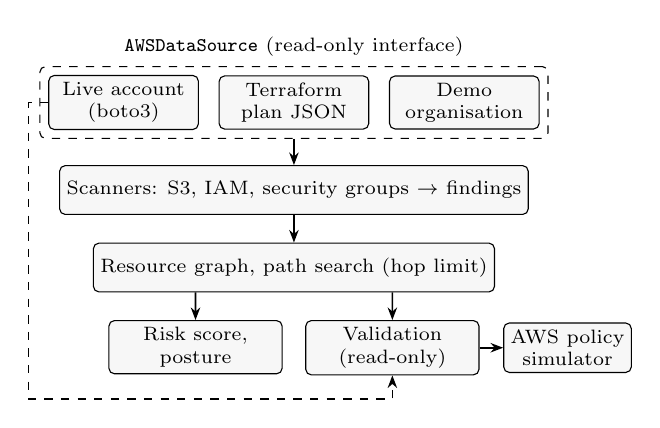
\begin{tikzpicture}[
  font=\scriptsize,
  box/.style={draw, rounded corners=2pt, align=center, minimum height=0.62cm, inner sep=2.5pt, fill=gray!6},
  arr/.style={-{Stealth[length=1.6mm]}, semithick}]
\node[box, minimum width=1.9cm] (live) {Live account\\(boto3)};
\node[box, minimum width=1.9cm, right=0.25cm of live] (plan) {Terraform\\plan JSON};
\node[box, minimum width=1.9cm, right=0.25cm of plan] (demo) {Demo\\organisation};
\node[draw, dashed, rounded corners=2pt, fit=(live)(plan)(demo), inner sep=3pt, label={[font=\scriptsize]above:\texttt{AWSDataSource} (read-only interface)}] (src) {};
\node[box, below=0.45cm of plan, minimum width=4.6cm] (scan) {Scanners: S3, IAM, security groups $\rightarrow$ findings};
\node[box, below=0.35cm of scan, minimum width=4.6cm] (graph) {Resource graph, path search (hop limit)};
\node[box, below=0.35cm of graph, minimum width=2.2cm, xshift=-1.25cm] (score) {Risk score,\\posture};
\node[box, below=0.35cm of graph, minimum width=2.2cm, xshift=1.25cm] (val) {Validation\\(read-only)};
\node[box, right=0.3cm of val, minimum width=1.3cm] (sim) {AWS policy\\simulator};
\draw[arr] (src.south) -- (scan.north);
\draw[arr] (scan) -- (graph);
\draw[arr] (graph.south) ++(-1.25,0) -- (score.north);
\draw[arr] (graph.south) ++(1.25,0) -- (val.north);
\draw[arr] (val) -- (sim);
\draw[arr, dashed] (live.west) -- ++(-0.25,0) coordinate (c1) |- ([yshift=-0.3cm]val.south) -- (val.south);
\end{tikzpicture}
\caption{CloudChain pipeline. All analysis runs against one read-only data-source interface; validation returns to the live account.}
\label{fig:arch}
\end{figure}

Fig.~\ref{fig:arch} shows the pipeline. Every scanner is written against a single interface, \texttt{AWSDataSource}, which exposes only read operations. Three implementations exist: a live account through boto3, a Terraform plan, and a seeded three-account demo organisation. Because the scanners never know which source they read, the analysis that gates a pull request is the same code that runs after deployment.

\subsection{Findings}
Scanners emit findings for S3 (public access, credential-shaped object keys in public buckets, encryption, versioning), IAM (missing MFA, stale keys, administrator-equivalent policies, escalation primitives, \texttt{iam:PassRole} combined with a compute-creation action, cross-account trust) and EC2 security groups open to the internet. Policies are read in full: attached AWS-managed, attached customer-managed and inline. Action patterns are matched with IAM's wildcard semantics, so a grant of \texttt{iam:*} or \texttt{iam:Pass*} covers \texttt{iam:PassRole}. An identity holding \texttt{iam:*} on all resources is treated as administrator-equivalent, because it can attach \texttt{AdministratorAccess} to itself in one call.

\subsection{Graph model}
Nodes are resources namespaced by account (\texttt{111111111111/iam\_user:svc}), and each account has its own administrator sink. Edges carry one of the following relations:
\begin{itemize}
\item \texttt{leaks\_credentials\_for}: a public bucket exposes an access key belonging to a user;
\item \texttt{can\_pass\_role\_to}: an identity holds \texttt{iam:PassRole} on a role and an action that creates compute (Lambda, EC2) to run as it;
\item \texttt{can\_assume\_cross\_account}: a role's trust policy names a principal in another account;
\item \texttt{can\_escalate\_to\_admin}: an identity holds an IAM write permission that lets it grant itself administrator access;
\item \texttt{grants\_admin\_access}: an identity holds an administrator-equivalent policy.
\end{itemize}
\texttt{iam:PassRole} is same-account by construction in AWS, so a \texttt{can\_pass\_role\_to} edge never crosses an account boundary. Crossing requires \texttt{sts:AssumeRole} against a trust policy. Keeping the two separate prevents chains that look plausible and cannot be walked; a unit test asserts it.

\subsection{Paths}
An \textit{attack path} starts at an entry point an unauthenticated attacker can reach (a public, sensitive resource) and ends at an administrator sink. An \textit{escalation route} starts at an ordinary identity and ends at a sink; it matters only once that identity is compromised. The two are reported and scored separately so that a latent primitive never scores as badly as an open door. Paths are enumerated with simple-path search bounded by a hop limit (default six), because the number of simple paths grows factorially on densely connected graphs (Section~\ref{sec:scale}).

\subsection{Opt-in credential correlation}
In the demo organisation the owner of a leaked key is known. On a real account, a key name such as \texttt{credentials.csv} does not say whose key it is. With an explicit opt-in flag, CloudChain reads the first 64\,KB of credential-shaped objects in public buckets, extracts access key IDs with a regular expression, and matches them against \texttt{iam:ListAccessKeys}. Secret keys are never extracted, object bytes are discarded after matching, and only masked IDs reach the report. Keys owned by another account are identified with \texttt{sts:GetAccessKeyInfo} and reported, not guessed at.

\section{Read-Only Path Validation}\label{sec:validation}

For each hop of a path, the validation engine runs a verifier specific to the edge relation, records every API call it made, and returns one of three verdicts:
\begin{itemize}
\item CONFIRMED: the API responses show the hop's precondition holds now;
\item REFUTED: a response contradicts it, so the path is stale or blocked;
\item UNVERIFIABLE: the responses were not enough to decide, for example because a read was denied.
\end{itemize}
A path is REFUTED if any hop is, CONFIRMED only if every hop is, and UNVERIFIABLE otherwise. Missing information never produces CONFIRMED.

\subsection{Verifiers}
The S3 hop re-reads the bucket's public access block, ACL and policy status, re-lists object keys, and checks that the leaked user still has an active access key. The PassRole hop re-reads the identity's policies and checks that \texttt{iam:PassRole} still covers the target role and that a compute-creation action is still granted. The self-escalation hop checks that at least one escalation primitive is still granted. The administrator hop checks for an administrator-equivalent statement. The cross-account hop re-reads the target role's trust policy in the account that owns the role.

\subsection{Second opinion from AWS}
Static analysis in CloudChain does not model explicit denies, permissions boundaries, SCPs or condition keys. After a static verifier confirms a permission hop, CloudChain calls \texttt{iam:SimulatePrincipalPolicy}~\cite{awssim} for the actions the hop needs. If the simulator denies them, the hop becomes REFUTED and the reason names the layer that blocked it (SCP, boundary or explicit deny). If a denial depends on a condition key the simulator has no value for, the hop becomes UNVERIFIABLE, not REFUTED. If the scanning identity may not call the simulator, the static verdict stands and the evidence says so.

The simulator also settles a case static analysis cannot. When an identity's own policies come back empty, the identity may have no permissions, the read may have been denied, or the grant may come from an IAM group that CloudChain's static reader does not resolve. The validator asks the simulator and reports REFUTED, CONFIRMED with a note about the indirect grant, or UNVERIFIABLE when no simulator is available.

\subsection{Safety}
Validation never performs an escalation: no role is assumed, no function created and no policy attached. Verifying that an identity \textit{can} pass a role into Lambda means confirming the grant, not using it. A CONFIRMED verdict therefore means every precondition holds now, which is weaker than a demonstrated exploit and stronger than configuration inference. The data-source methods validation may call are listed in an allowlist, and a test wraps the data source in a tripwire that fails the build if validation calls anything else, including the opt-in object read. Every recorded call carries its \texttt{aws} CLI equivalent so a reviewer can reproduce the verdict by hand.

\section{Scoring}\label{sec:scoring}

Each finding receives a contextual score
\begin{equation}
s = w_{\mathit{sev}} \cdot m_{\mathit{net}} \cdot m_{\mathit{sens}} \cdot m_{\mathit{path}},
\end{equation}
where $w_{\mathit{sev}} \in \{1, 3, 6, 10\}$ for LOW to CRITICAL, $m_{\mathit{net}} = 1.5$ if the resource is internet-facing, $m_{\mathit{sens}} = 1.5$ if it holds credentials or sensitive data, and $m_{\mathit{path}} = 2.5$ if it lies on an internet-reachable attack path; each multiplier is 1 otherwise. The interface shows the chain of multipliers for every finding.

The account posture score starts at 100 and subtracts four dimension deductions: exposure (up to 25 points, internet-facing findings weighted by severity), privilege (up to 25, identity weaknesses weighted by how far they advance an attacker), reachability (up to 30, from the existence and shape of routes to administrator access) and blast radius (up to 20, the fraction of the graph reachable from exposed entry points). Each dimension publishes its formula and the findings behind it, and a test asserts that the headline number always equals 100 minus the published deductions. A confirmed internet-reachable route to administrator access caps the grade at F.

\section{Implementation}

CloudChain is written in Python with FastAPI, networkx~\cite{networkx} for the graph and boto3 for AWS access, with a React front end and a command-line interface that runs scans, validations and Terraform plan checks without the server. The test suite has 226 tests covering scanners, graph construction, path search, scoring, the posture contract, validation verdicts and safety, credential handling and the plan gate. Continuous integration runs the suite on Python 3.10 and 3.13, runs a demo scan on a clean machine, and checks that the plan gate blocks a known-dangerous Terraform plan. Submitted credentials are held in memory for one scan, never persisted, and never returned to the browser; a test asserts the last property.

\section{Evaluation}\label{sec:eval}

We asked four questions. Does CloudChain find the escalation-capable identities a mature scanner finds (RQ1)? Does validation separate routes that can be walked from routes that cannot (RQ2)? Does re-validation notice when a route is fixed (RQ3)? How do run time and the scores behave as inputs change (RQ4)?

\subsection{Setup}
We used a real AWS account that belongs to an AWS Organization. The organisation applies an SCP that explicitly denies, among others, \texttt{lambda:CreateFunction}, \texttt{s3:CreateBucket}, \texttt{ec2:RunInstances} and \texttt{ec2:DescribeSecurityGroups}, which we confirmed with the policy simulator before the experiment. The SCP rules out S3, EC2 and Lambda resources, so the evaluation covers IAM only. Scans used a dedicated user with the AWS-managed \texttt{SecurityAudit} policy plus \texttt{iam:SimulatePrincipalPolicy}.

A script in the repository creates nine test users, each with a single inline policy, and two roles: one with \texttt{AdministratorAccess} and one with no permissions, both trusting Lambda. Table~\ref{tab:testbed} lists the users. Six hold an escalation capability; three are negative controls. Four management roles created by the organisation were present in the account and were marked as known-benign through CloudChain's suppression setting, which downgrades and annotates findings instead of hiding them.

\subsection{RQ1: Detection compared with Prowler}
On the empty account, before the testbed existed, CloudChain reported 8 findings and no paths. Four were on the organisation's management roles and were suppressed as above; the rest (an administrator user, two users without MFA and a missing password policy) were correct.

With the testbed in place, CloudChain reported 7 escalation routes from the 6 escalation-capable users. The wildcard user produced two routes, one to the testbed's administrator role and one to an organisation role that also holds administrator access. Prowler 5 with its IAM checks flagged the same 6 users through its \texttt{iam\_inline\_policy\_allows\_\allowbreak privilege\_escalation} check. Neither tool reported an escalation for the three negative controls (Table~\ref{tab:testbed}). The user allowed to pass only the harmless role received a CRITICAL escalation finding from CloudChain's IAM scanner, but the graph produced no route for it, because the role it can pass is not administrator-equivalent.

Prowler failed 53 checks in total and took 1\,min 45\,s; CloudChain reported 24 findings. Raw finding counts are not directly comparable, because Prowler includes checks CloudChain does not implement (for example, confused-deputy protection on service roles).

\begin{table}[t]
\caption{Testbed identities and outcomes. P = Prowler escalation finding; S = CloudChain routes from static analysis; V = CloudChain validation verdict ($\dagger$ blocked by the organisation's SCP).}
\label{tab:testbed}
\centering
\footnotesize
\setlength{\tabcolsep}{2.5pt}
\begin{tabular}{@{}llccl@{}}
\toprule
User & Inline policy grants & P & S & V \\
\midrule
attach & \texttt{iam:AttachUserPolicy} & yes & 1 & CONFIRMED \\
policyver & \texttt{iam:CreatePolicyVersion} & yes & 1 & CONFIRMED \\
putpolicy & \texttt{iam:PutUserPolicy} & yes & 1 & CONFIRMED \\
addgroup & \texttt{iam:AddUserToGroup} & yes & 1 & REFUTED$^\dagger$ \\
passrole-lambda & PassRole (admin) + Lambda & yes & 1 & REFUTED$^\dagger$ \\
wildcard-pass & \texttt{iam:Pass*}, \texttt{lambda:Create*} & yes & 2 & REFUTED$^\dagger$ \\
passrole-scoped & PassRole (harmless) + Lambda & no & 0 & n/a \\
readonly & \texttt{iam:Get*}, \texttt{iam:List*} & no & 0 & n/a \\
s3only & \texttt{s3:*} & no & 0 & n/a \\
\bottomrule
\end{tabular}
\end{table}

\subsection{RQ2: Validation under an SCP}
Validation confirmed 3 of the 7 routes and refuted 4. Three refutations came from the SCP's denial of the Lambda actions the PassRole routes need. The fourth, \texttt{iam:AddUserToGroup}, was denied by the same SCP; we had not known this before the run, and the simulator reported it. In each case the static verifier had confirmed the grant, and the simulator overturned it with the reason ``a service control policy, an explicit Deny''. A configuration-only analysis would have reported all 7 routes as open. Prowler reported all 6 users at the same HIGH severity and did not indicate that 4 of them could not escalate in this account.

\subsection{RQ3: Detecting stale paths}
We then removed the escalation permission from two users (attach and putpolicy) and re-ran validation on the stored scan without rescanning. Both routes changed from CONFIRMED to REFUTED. The policyver route, left untouched as a control, stayed CONFIRMED, and the four SCP-blocked routes stayed REFUTED.

The first attempt at this experiment exposed a defect: with the users' only policy deleted, the validator could not tell an identity with no policies from a read it was not allowed to make, and returned UNVERIFIABLE. We changed the validator to settle that case with the policy simulator (Section~\ref{sec:validation}), added tests for it, and re-ran the same validation, which produced the results above.

\subsection{RQ4a: Scalability}\label{sec:scale}
We generated seeded three-account organisations with 30 to 10{,}000 identities and a fixed mix of administrators, escalation primitives, PassRole grants, cross-account trust and leaking public buckets, and timed the full offline pipeline (median of three runs; AWS API latency excluded). Fig.~\ref{fig:scale}(a) and Table~\ref{tab:scale} show the results. At 10{,}000 identities the analysis took 2.6\,s and the longest route had five hops, so the hop limit of six never cut a route and made no measurable difference to run time.

The limit matters on dense graphs. Fig.~\ref{fig:scale}(b) shows a worst case in which every identity can reach every other and one can escalate. Unbounded enumeration found 109{,}601 routes in 7.9\,s at 9 identities and exceeded 60\,s at 10. With a limit of six, 12 identities took 7.0\,s.

The more pressing limit at scale is the number of routes, not time: 43{,}752 at 10{,}000 identities, mostly from wildcard PassRole grants that reach every administrator role. No analyst can read that many, which argues for grouping routes by shared hops.

\begin{figure}[t]
\centering
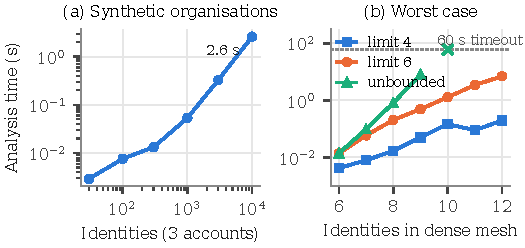
\includegraphics[width=\columnwidth]{fig_scalability.pdf}
\caption{(a) End-to-end analysis time on synthetic organisations, hop limit 6. (b) Path search on a fully connected trust mesh; the unbounded search timed out at 10 identities.}
\label{fig:scale}
\end{figure}

\begin{table}[t]
\caption{Synthetic organisations (hop limit 6, median of 3 runs)}
\label{tab:scale}
\centering
\footnotesize
\begin{tabular}{@{}rrrrrr@{}}
\toprule
Identities & Findings & Edges & Attack & Escalation & Time (s) \\
\midrule
30 & 29 & 12 & 0 & 3 & 0.003 \\
300 & 179 & 101 & 1 & 69 & 0.013 \\
1{,}000 & 617 & 436 & 0 & 293 & 0.054 \\
3{,}000 & 1{,}931 & 3{,}540 & 83 & 3{,}125 & 0.33 \\
10{,}000 & 6{,}394 & 44{,}224 & 860 & 42{,}892 & 2.6 \\
\bottomrule
\end{tabular}
\end{table}

\subsection{RQ4b: Sensitivity to the weights}\label{sec:sensitivity}
Every weight in both scores was chosen by hand, so we measured how much they drive the output. We scaled each weight by 0.5, 0.75, 1.25 and 1.5 in turn and compared the result with the baseline on the demo organisation and ten synthetic organisations of 300 identities. For finding scores we report Kendall's $\tau$~\cite{kendall1938} between baseline and perturbed scores and the share of the baseline top ten that remained in the top ten. For the posture score we report the mean absolute change and the share of organisations whose letter grade changed. Table~\ref{tab:sens} gives the worst case over the four factors.

Finding rankings were stable under the multipliers: mean $\tau$ stayed at or above 0.95 and the lowest single-organisation $\tau$ was 0.84. The largest change came from halving the CRITICAL base weight, which places CRITICAL below HIGH ($\tau_{\min} = 0.79$, top-ten overlap 0.55); that perturbation inverts the severity scale rather than tuning it. The posture score was more sensitive. Scaling the exposure, privilege or reachability weight by 0.5 or 1.5 moved the score by 10 to 13 points on average and changed the grade in up to 36\% of organisations. The score's decomposition makes that dependence visible, but the absolute value should be read as relative to the chosen weights until they are calibrated against incident data.

\begin{table}[t]
\caption{Weight sensitivity, worst case over factors 0.5, 0.75, 1.25, 1.5}
\label{tab:sens}
\centering
\footnotesize
\setlength{\tabcolsep}{3pt}
\begin{tabular}{@{}lcccc@{}}
\toprule
Weight & $\tau_{\min}$ & Top-10 & $|\Delta|$ posture & Grade changed \\
\midrule
Internet-facing multiplier & 0.84 & 0.76 & 0 & 0\% \\
Sensitive multiplier & 0.95 & 0.84 & 0 & 0\% \\
Attack-path multiplier & 0.86 & 0.93 & 0 & 0\% \\
CRITICAL base weight & 0.79 & 0.55 & 0 & 0\% \\
HIGH base weight & 0.92 & 0.74 & 0 & 0\% \\
Exposure weight & 1.00 & 1.00 & 11.2 & 36\% \\
Privilege weight & 1.00 & 1.00 & 12.6 & 36\% \\
Reachability weight & 1.00 & 1.00 & 9.9 & 36\% \\
Blast-radius weight & 1.00 & 1.00 & 0.6 & 9\% \\
Escalation-only floor & 1.00 & 1.00 & 2.5 & 27\% \\
\bottomrule
\end{tabular}
\end{table}

\section{Limitations}

The real-account evaluation covers IAM only, because the organisation's SCP denies the S3, EC2 and Lambda actions needed to build other scenarios. The internet-to-administrator chain through a leaking bucket is exercised by unit tests and the demo organisation but not on a live account. The testbed has nine identities that we designed, so it shows that the mechanisms work, not how often they matter in production estates.

Real-mode scans cover a single account. The graph model is organisation-wide and the demo exercises three accounts, but scanning a live organisation needs an \texttt{sts:AssumeRole} fan-out from a management-account role that CloudChain does not perform.

The static reader does not resolve permissions granted through IAM groups, resource-based policies other than bucket and trust policies, or condition keys. The simulator compensates during validation, but only when the scanning identity is allowed to call it, and the simulator itself does not evaluate resource-based policies for roles~\cite{awssim}. The \texttt{iam:AddUserToGroup} edge is drawn without checking that a more privileged group exists, which over-approximates.

The posture weights are not calibrated against incident data, and the sensitivity analysis shows the letter grade depends on them. Route counts grow quickly with wildcard PassRole grants.

\section{Conclusion}

CloudChain derives attack paths from AWS configuration and then tests them against the account with read-only calls and AWS's policy simulator. On an SCP-governed account it matched Prowler's detection of escalation-capable identities and went further in one respect that matters to an analyst: it showed that four of seven derived routes could not be walked, and it recognised two routes as fixed without a rescan. Future work is a live multi-account scan through role assumption, grouping of routes that share hops, resolution of group and resource policies in the static reader, broader service coverage on an account without restrictive SCPs, and calibration of the posture weights.

\begin{thebibliography}{00}
\bibitem{prowler} Prowler, ``Prowler: open source cloud security platform,'' GitHub repository. [Online]. Available: \url{https://github.com/prowler-cloud/prowler}
\bibitem{scoutsuite} NCC Group, ``ScoutSuite: multi-cloud security auditing tool,'' GitHub repository. [Online]. Available: \url{https://github.com/nccgroup/ScoutSuite}
\bibitem{pmapper} NCC Group, ``Principal Mapper (PMapper),'' GitHub repository. [Online]. Available: \url{https://github.com/nccgroup/PMapper}
\bibitem{awspx} WithSecure Labs, ``awspx: a graph-based tool for visualizing effective access and resource relationships in AWS,'' GitHub repository. [Online]. Available: \url{https://github.com/WithSecureLabs/awspx}
\bibitem{cartography} Cartography project, ``Cartography,'' GitHub repository. [Online]. Available: \url{https://github.com/cartography-cncf/cartography}
\bibitem{cloudsplaining} Salesforce, ``Cloudsplaining: AWS IAM security assessment tool,'' GitHub repository. [Online]. Available: \url{https://github.com/salesforce/cloudsplaining}
\bibitem{bloodhound} SpecterOps, ``BloodHound,'' GitHub repository. [Online]. Available: \url{https://github.com/SpecterOps/BloodHound}
\bibitem{gietzen2018} S. Gietzen, ``AWS IAM privilege escalation: methods and mitigation,'' Rhino Security Labs, 2018. [Online]. Available: \url{https://rhinosecuritylabs.com/aws/aws-privilege-escalation-methods-mitigation/}
\bibitem{sheyner2002} O. Sheyner, J. Haines, S. Jha, R. Lippmann, and J. M. Wing, ``Automated generation and analysis of attack graphs,'' in \textit{Proc. IEEE Symp. Security and Privacy}, 2002, pp. 273--284.
\bibitem{mulval} X. Ou, S. Govindavajhala, and A. W. Appel, ``MulVAL: a logic-based network security analyzer,'' in \textit{Proc. 14th USENIX Security Symp.}, 2005.
\bibitem{ou2006} X. Ou, W. F. Boyer, and M. A. McQueen, ``A scalable approach to attack graph generation,'' in \textit{Proc. 13th ACM Conf. Computer and Communications Security (CCS)}, 2006, pp. 336--345.
\bibitem{zelkova} J. Backes et al., ``Semantic-based automated reasoning for AWS access policies using SMT,'' in \textit{Proc. Formal Methods in Computer Aided Design (FMCAD)}, 2018.
\bibitem{awssim} Amazon Web Services, ``SimulatePrincipalPolicy,'' AWS Identity and Access Management API Reference. [Online]. Available: \url{https://docs.aws.amazon.com/IAM/latest/APIReference/API_SimulatePrincipalPolicy.html}
\bibitem{awseval} Amazon Web Services, ``Policy evaluation logic,'' AWS IAM User Guide. [Online]. Available: \url{https://docs.aws.amazon.com/IAM/latest/UserGuide/reference_policies_evaluation-logic.html}
\bibitem{awsscp} Amazon Web Services, ``Service control policies (SCPs),'' AWS Organizations User Guide. [Online]. Available: \url{https://docs.aws.amazon.com/organizations/latest/userguide/orgs_manage_policies_scps.html}
\bibitem{networkx} A. A. Hagberg, D. A. Schult, and P. J. Swart, ``Exploring network structure, dynamics, and function using NetworkX,'' in \textit{Proc. 7th Python in Science Conf. (SciPy)}, 2008, pp. 11--15.
\bibitem{kendall1938} M. G. Kendall, ``A new measure of rank correlation,'' \textit{Biometrika}, vol. 30, no. 1/2, pp. 81--93, 1938.
\bibitem{cloudchain} CloudChain, GitHub repository. [Online]. Available: \url{https://github.com/threetheodrummer/CloudChain}
\end{thebibliography}

\end{document}
